% \usepackage{xcolor}
% \usepackage{afterpage}
% \usepackage{pifont,mdframed}
% \usepackage{wrapfig}
% \usepackage[bottom]{footmisc}

\makeatletter
\gdef\this@inputfilename{input.txt}
\gdef\this@outputfilename{output.txt}
\makeatother

\newcommand{\inputfile}{\texttt{input.txt}}
\newcommand{\outputfile}{\texttt{output.txt}}

\newenvironment{warning}
  {\par\begin{mdframed}[linewidth=2pt,linecolor=gray]%
    \begin{list}{}{\leftmargin=1cm
                   \labelwidth=\leftmargin}\item[\Large\ding{43}]}
  {\end{list}\end{mdframed}\par}

Al corso di \emph{Ittiologia Computazionale} Gabriele sta studiando le dinamiche algoritmiche del mondo dei pesci. Un argomento particolarmente interessante è quello dell'alimentazione dei \emph{Pesci Mangioni}.

\begin{wrapfigure}{r}{5cm}
\centering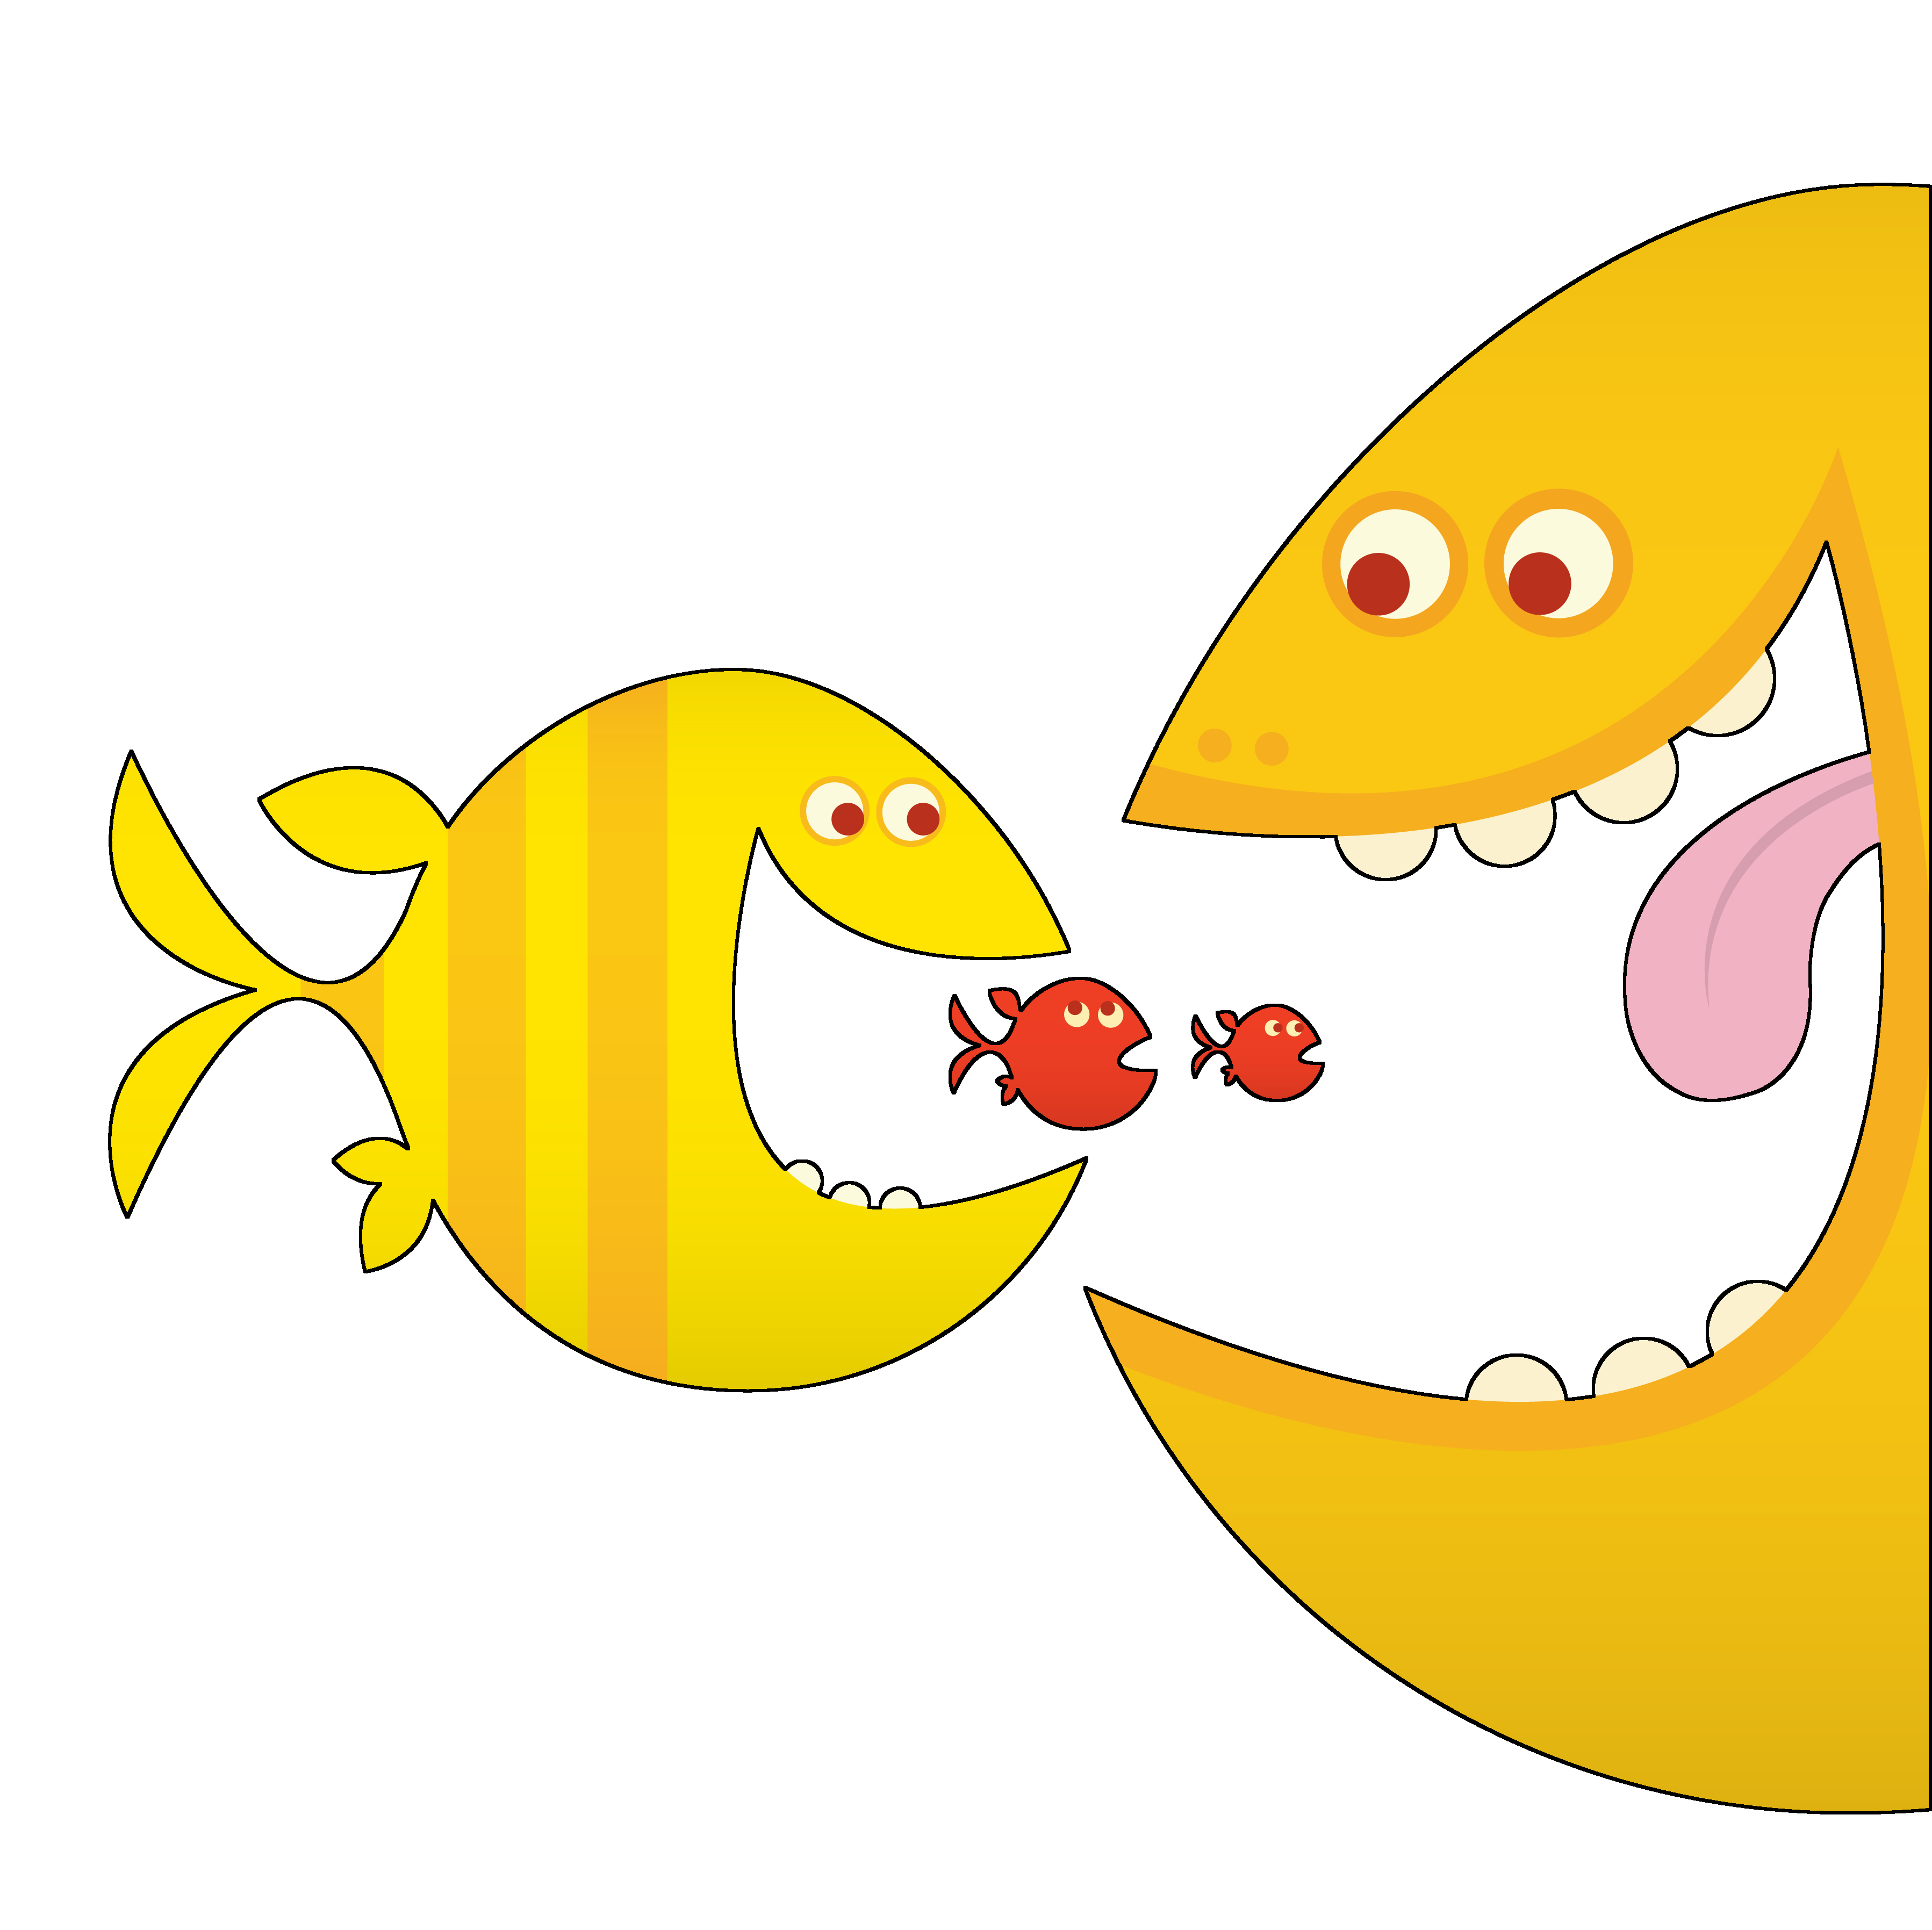
\includegraphics[width=5cm]{pesci.jpg}
\end{wrapfigure}

Questi voracissimi pesci, di dimensioni molto variegate, sono molto aggressivi e ogni volta che si sentono osservati da un'altro pesce reagiscono mangiandoselo (se possono), senza mai sentire il senso di sazietà. Per compito Gabriele ha stilato un modello semplificato del loro comportamento, che dovrebbe essere valido almeno nel caso in cui i pesci si trovino in un tubo da sperimentazione. Secondo il modello:

\begin{itemize}[nolistsep, itemsep=2mm]
	\item ogni pesce può nuotare da sinistra verso destra o da destra verso sinistra, e stando nel tubo questa direzione non cambierà mai,
	\item ogni pesce ha una grandezza ben definita, e tutte le grandezze sono distinte,
	\item un incrocio di pesci è una coppia di pesci adiacenti, per cui il più a sinistra nuota verso destra, e il più a destra nuota verso sinistra,
	\item durante un incrocio di pesci il pesce più grande mangia il pesce più piccolo e continua nel suo moto, eventualmente incrociando altri pesci.
\end{itemize}

Per verificare quanto è buono il modello che ha derivato di questa specie curiosa, Gabriele intende ora liberare in un tubo $N$ Pesci Mangioni e monitorare cosa succede. Quanti pesci dovrebbero rimanere vivi dopo che tutti gli incroci si saranno risolti?

\Implementation
Dovrai sottoporre esattamente un file con estensione \texttt{.c}, \texttt{.cpp} o \texttt{.pas}.

\begin{warning}
Tra gli allegati a questo task troverai un template (\texttt{pesci.c}, \texttt{pesci.cpp}, \texttt{pesci.pas}) con un esempio di implementazione da completare.
\end{warning}

Se sceglierai di utilizzare il template, dovrai implementare la seguente funzione:
\begin{center}\begin{tabularx}{\textwidth}{|c|X|}
\hline
C/C++  & \verb|int mangia(int N, int direzione[], int dimensione[]);|\\
\hline
Pascal & \small\verb|function mangia(N: longint; var direzione, dimensione: array of longint): longint;|\\
\hline
\end{tabularx}\end{center}
In cui:
\begin{itemize}[nolistsep]
  \item L'intero $N$ rappresenta il numero di pesci liberati da Gabriele.
  \item L'array \texttt{direzione}, indicizzato da $0$ a $N-1$, indica se l'$i-$esimo pesce nuota da sinistra verso destra (\texttt{direzione[$i$]}$= 0$) o da destra verso sinistra (\texttt{direzione[$i$]}$= 1$).
  \item L'array \texttt{dimensione}, indicizzato da $0$ a $N-1$, indica la dimensione dell'$i-$esimo pesce.
  \item La funzione dovrà restituire il numero di Pesci Mangioni sopravvissuti dopo che tutti gli incroci sono stati risolti, che verrà stampato sul file di output.
\end{itemize}

\InputFile
Il file \inputfile{} è composto da $N+1$ righe. La prima riga contiene l'unico intero $N$. Le successive $N$ righe contengono ciascuna i due interi \texttt{direzione[$i$]}, \texttt{dimensione[$i$]}.

\OutputFile
Il file \outputfile{} è composto da un'unica riga contenente un unico intero, la risposta a questo problema.

% Assunzioni
\Constraints
\begin{itemize}[nolistsep, itemsep=2mm]
	\item $1 \le N \le 100\,000$.
	\item $\texttt{direzione}[i] \in \{0, 1\}$ per ogni $i=0\ldots N-1$.
	\item $1 \le \texttt{dimensione}[i] \le 10^9$ per ogni $i=0\ldots N-1$; inoltre, le dimensioni dei pesci sono tutte distinte.
\end{itemize}

\Scoring
Il tuo programma verrà testato su diversi test case raggruppati in subtask.
Per ottenere il punteggio relativo ad un subtask, è necessario risolvere
correttamente tutti i test relativi ad esso.

\begin{itemize}[nolistsep,itemsep=2mm]
  \item \textbf{\makebox[2cm][l]{Subtask 1} [10 punti]}: Casi d'esempio.
  \item \textbf{\makebox[2cm][l]{Subtask 2} [20 punti]}: $N \leq 10$.
  \item \textbf{\makebox[2cm][l]{Subtask 3} [40 punti]}: $N \leq 100$.
  \item \textbf{\makebox[2cm][l]{Subtask 4} [30 punti]}: Nessuna limitazione specifica.
\end{itemize}

% Esempi
\Examples
\begin{example}
\exmp{
2
0 6
1 9
}{%
1
}%
\end{example}
\begin{example}
\exmp{
2
1 6
1 9
}{%
2
}%
\end{example}
\begin{example}
\exmp{
5
0 12
0 9
1 3
0 4
1 6
}{%
2
}%
\end{example}

\pagebreak
\Explanation
Nel \textbf{primo caso di esempio} il secondo pesce, di dimensione 9, mangia il primo, di dimensione 6.\\[2mm]
Nel \textbf{secondo caso di esempio} i pesci non si incrociano.\\[2mm]
Nel \textbf{terzo caso di esempio} il pesce di dimensione 4 viene mangiato dal pesce di dimensione 6, ma il pesce di dimensione 9 mangia sia il pesce di dimensione 3 che quello di dimensione 6.